\documentclass{beamer}
\usetheme{Antibes}
\usepackage{xcolor, colortbl}
\usepackage{algorithm}
\usepackage{algpseudocode}
\usepackage{textcomp}
\usepackage{listings}
\usepackage{hyperref}
\usepackage{alltt}
\usepackage{tikz}
\usepackage{framed}
\usepackage{marvosym}
\usepackage{wasysym}
\usepackage{marvosym}
\usepackage{crayola}
\usepackage{mathpartir}
\usepackage{tabularx}
\usepackage[belowskip=-15pt,aboveskip=0pt]{caption}
\usepackage[skins]{tcolorbox}
\usepackage{multicol}
\usetikzlibrary{positioning,shapes,arrows, backgrounds, fit, shadows, automata}
\usetikzlibrary{decorations.markings, calc}
%\usepackage{wasysym}
%\usepackage{marvosym}
\setbeamertemplate{footline}[frame number]
%\usecolortheme{fly}
\usefonttheme{serif}

\title[Sujit]{Lexical Analysis \\
Programming Languages}
\author{Sujit Kumar Chakrabarti}
\institute{IIITB}
\date{}


\definecolor{lightblue}{rgb}{0.8,0.93,1.0} % color values Red, Green, Blue
\definecolor{darkblue}{rgb}{0.4,0.3,1.0} % color values Red, Green, Blue
\definecolor{Blue}{rgb}{0,0,1.0} % color values Red, Green, Blue
\definecolor{darkgreen}{rgb}{0,0.7,0.2} % color values Red, Green, Blue
\definecolor{Red}{rgb}{1,0,0} % color values Red, Green, Blue
\definecolor{Pink}{rgb}{0.7,0,0.2}
\definecolor{links}{HTML}{2A1B81}
\definecolor{mydarkgreen}{HTML}{126215}
\newcommand{\highlight}[1]{{\color{Red}(#1)}}

\newcommand{\myheader}[1]{
	{\color{darkblue}
		\begin{Large}
			\begin{center}
				{#1}
			\end{center}
		\end{Large}
	}
}
\newcommand{\myminorheader}[1]{
	{\color{BrickRed}
		\begin{Large}
			{\fontfamily{\sfdefault}\selectfont\textbf{#1}}
		\end{Large}
	}
}

%\tikzstyle{input} = [coordinate]
%\tikzstyle{output} = [coordinate]


\tikzstyle{bb}=[%
      rectangle, draw=black, thick, fill=OliveGreen!30, drop shadow, align=center,
      text ragged, minimum height=2em, minimum width=2em, inner sep=6pt
]

\tikzstyle{inv}=[%
      rectangle, draw=none,  align=center,
      text ragged, minimum height=2em, minimum width=2em, align=center, inner sep=6pt
]

\tikzstyle{db}=[%
      ellipse, draw=black, thick, fill=pink, drop shadow, align=center,
      text ragged, minimum height=2em, inner sep=6pt
]

\tikzstyle{jn}=[%
      inner sep=0cm, outer sep=0cm
]

\tikzstyle{io}=[%
      trapezium, trapezium left angle=60, trapezium right angle=120, draw=black, thick, fill=brown, drop shadow,
      text ragged, minimum height=2em, minimum width=2em, inner sep=6pt, align=center
]

\tikzstyle{glio}=[%
      trapezium, trapezium left angle=60, trapezium right angle=120, draw=red, line width = 1mm, fill=brown, drop shadow,
      text ragged, minimum height=2em, minimum width=2em, inner sep=6pt
]
\tikzstyle{gl}=[%
      rectangle, draw=red, line width = 1mm, fill=lightblue, drop shadow,
      text ragged, minimum height=2em, minimum width=2em, inner sep=6pt
]

\tikzstyle{en}=[%
      rectangle, draw=black, thick, fill=none,
      text ragged, minimum height=2em, minimum width=2em, inner sep=6pt
]

\tikzstyle{sh}=[%
      rectangle, draw=gray, thick, fill=none, color = gray,
      text ragged, minimum height=2em, minimum width=2em, inner sep=6pt
]


\lstdefinestyle{javacode}{
	language = Java,
	basicstyle = \ttfamily\scriptsize,
	stringstyle = \ttfamily,
	keywordstyle=\color{Blue}\bfseries,
	identifierstyle=\color{Pink},
	commentstyle=\color{darkgreen},
	frame=single,
	frameround=tttt,
%	numbers=left
	showstringspaces=false
}

\lstdefinestyle{camlcode}{
	language = Caml,
	basicstyle = \scriptsize\ttfamily,
	stringstyle = \color{red}\ttfamily,
	keywordstyle=\color{Blue}\bfseries,
	identifierstyle=\ttfamily,
	frame=single,
	frameround=tttt,
	numbers=none,
	showstringspaces=false,
	escapeinside={(*@}{@*)}
}

\lstdefinestyle{outputcode}{
	language = bash,
	backgroundcolor = \color{black},
	basicstyle = \tiny\ttfamily\color{white},
	stringstyle = \color{red}\ttfamily,
	keywordstyle=\color{white}\bfseries,
	identifierstyle=\ttfamily,
	frameround=tttt,
	numbers=none,
	showstringspaces=false,
	escapeinside={(*@}{@*)}
}

\newtcolorbox{myframe}[2][]{%
  enhanced,colback=white,colframe=black,coltitle=black,
  sharp corners,boxrule=0.4pt,
  fonttitle=\itshape,
  attach boxed title to top left={yshift=-0.3\baselineskip-0.4pt,xshift=2mm},
  boxed title style={tile,size=minimal,left=0.5mm,right=0.5mm,
    colback=white,before upper=\strut},
  title=#2,#1
}

\begin{document}
\maketitle

\section{Manual Implementation of Lexical Analysis}

% frame begin %%%%%%%%%%%%%%%%%%%%%%%%
\begin{frame}{Manual Implementation of Lexical Analysis}
{Section Goals}
\begin{enumerate}
	\item How FSAs come together to build a complete lexical analyser
	\item Functional programming
	\item Software design: modularity, testability, scalability
\end{enumerate}
\end{frame}
% frame end %%%%%%%%%%%%%%%%%%%%%%%%


% frame begin %%%%%%%%%%%%%%%%%%%%%%%%
\begin{frame}{Manual Implementation of Lexical Analysis}
{Functional Programming -- Paradigm shift in Programming}
\begin{enumerate}
	\item Takes work to get the program to compile
	\item Requires very little time to test and debug
	\item Terse, expressive and maintenable
	\item Type system does the heavylifting
	\item Useful in system programming
\end{enumerate}
\end{frame}
% frame end %%%%%%%%%%%%%%%%%%%%%%%%


% frame begin %%%%%%%%%%%%%%%%%%%%%%%%
\begin{frame}{Manual Implementation of Lexical Analysis}
{The Lexer Algorithm}
\begin{tiny}
\begin{algorithmic}[0]
\Procedure{lexer}{$buffer$}
  \State $C \gets$ all scanners
  \State $S \gets \{\}$
  \While{there is input left}
    \State $c, la \gets$ \Call{nextChar}{$buffer$}
	\State $S$ $\gets$ all $s \in C$ terminating in success
	\State $C$ $\gets$ all $s \in C$ making a move
	\If{$C = \{\}$}
		\If{$S \neq \{\}$}
			\State choose randomly from $S$ and return corresponding token
		\Else
			\State raise $LexicalError$
		\EndIf
	\EndIf
  \EndWhile
\EndProcedure
\end{algorithmic}
\end{tiny}

\end{frame}
% frame end %%%%%%%%%%%%%%%%%%%%%%%%

% frame begin %%%%%%%%%%%%%%%%%%%%%%%%
\begin{frame}{Implementation of Lexical Analysis}
{Manual Implementation of Lexical Analysers -- Example}
\begin{center}
\begin{tabular}{|c|c|c|c|c|c|c|c|}
\hline
\cellcolor{red!75}i & \cellcolor{red!25}n & t & e & g & r & a & l \\
\hline
\end{tabular}
\end{center}

\begin{center}
\resizebox{0.7\textwidth}{!}{%
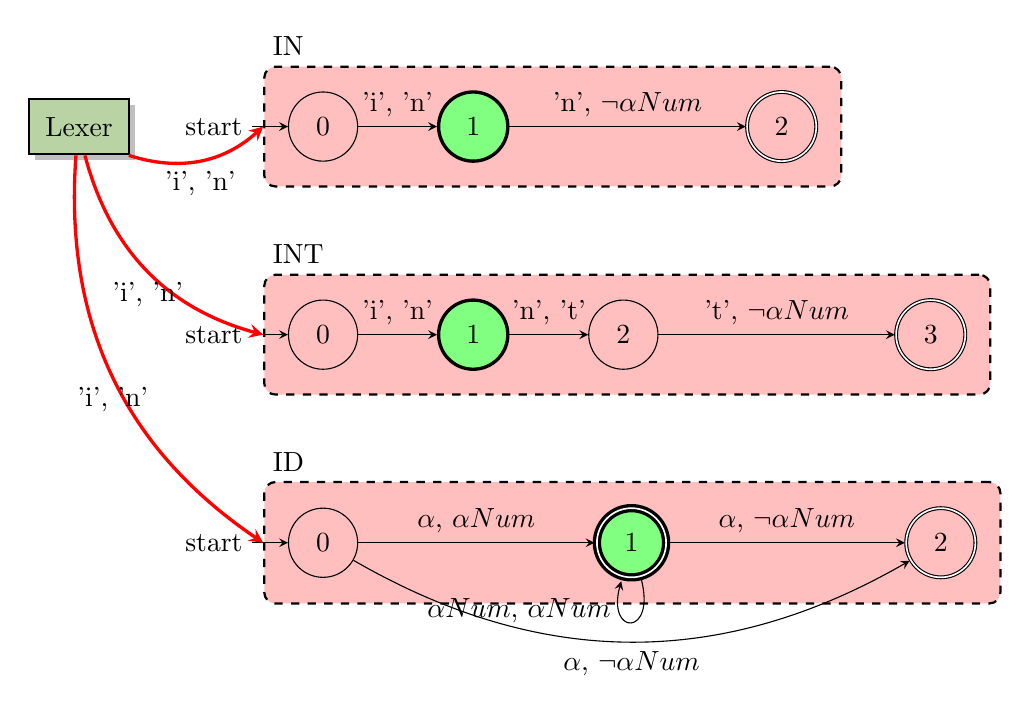
\begin{tikzpicture}[auto,
    ->,
    >=stealth,
    ,
    dead/.style={%
      rectangle, rounded corners=1.5mm, draw=gray, thick, fill=gray!25, drop shadow,align=center,
      text ragged, minimum height=2em, minimum width=2em, inner sep=6pt, outer sep=3pt
    },
    fun/.style = {%
      dashed, draw=black, thick, fill=red!25, rounded corners, rectangle, inner sep=.3cm
    },
    deadfun/.style = {%
      dashed, draw=gray, thick, fill=gray!25, rounded corners, rectangle, inner sep=.3cm
    }
  ]

    \node[bb] (lexer)                           {Lexer};
% IN  
    \node[initial, state]   (10) [right = of lexer, xshift=1cm]          {$0$};
    \node[state, very thick, fill=green!50]            (11) [right = of 10]             {$1$};
    \node[state, accepting] (12) [right = of 11, xshift=2cm] {$2$};
    
    \path (10) edge node {'i', 'n'} (11)
          (11) edge node {'n', $\neg\alpha Num$} (12)
    ;

% INT
    \node[initial, state]   (20) [below = of 10, yshift = -0.75cm] {$0$};
    \node[state, very thick, fill=green!50]            (21) [right = of 20] {$1$};
    \node[state]            (22) [right = of 21] {$2$};
    \node[state, accepting] (23) [right = of 22, xshift=2cm] {$3$};
    
    \path (20) edge node {'i', 'n'} (21)
          (21) edge node {'n', 't'} (22)
          (22) edge node {'t', $\neg\alpha Num$} (23)
    ;
    
%ID
    \node[initial, state]   (30) [below = of 20, yshift = -0.75cm] {$0$};
    \node[state, accepting, very thick, fill=green!50]            (31) [right = of 30, xshift=2cm] {$1$};
    \node[state, accepting]            (32) [right = of 31, xshift=2cm] {$2$};
    
    \path (30) edge node {$\alpha$, $\alpha Num$} (31)
          (31) edge[loop below] node[near end, left] {$\alpha Num$, $\alpha Num$} (31)
          (31) edge node[above] {$\alpha$, $\neg\alpha Num$} (32)
          (30) edge[bend right] node[below] {$\alpha$, $\neg\alpha Num$} (32)
    ;
    
    \begin{pgfonlayer}{background}
      \node[fun] (in)[fit = (10) (11) (12)] {};
      \node[fun] (int)[fit = (20) (21) (22) (23)] {};
      \node[fun] (id)[fit = (30) (31) (32)] {};
      \node[above right] at (in.north west){IN};
      \node[above right] at (int.north west){INT};
      \node[above right] at (id.north west){ID};

    \end{pgfonlayer}
    
	\draw[->, very thick, red, bend right] (lexer) to node[below, black]{'i', 'n'} (in.west);
	\draw[->, very thick, red, bend right] (lexer) to node[below, black]{'i', 'n'} (int.west);
	\draw[->, very thick, red, bend right] (lexer) to node[below, black]{'i', 'n'} (id.west);
	    
  \end{tikzpicture}
}

\end{center}

\end{frame}
% frame end %%%%%%%%%%%%%%%%%%%%%%%%


% frame begin %%%%%%%%%%%%%%%%%%%%%%%%
\begin{frame}{Implementation of Lexical Analysis}
{Manual Implementation of Lexical Analysers -- Example}
\begin{center}
\begin{tabular}{|c|c|c|c|c|c|c|c|}
\hline
i & \cellcolor{red!75}n & \cellcolor{red!25}t & e & g & r & a & l \\
\hline
\end{tabular}
\end{center}

\begin{center}
\resizebox{0.7\textwidth}{!}{%
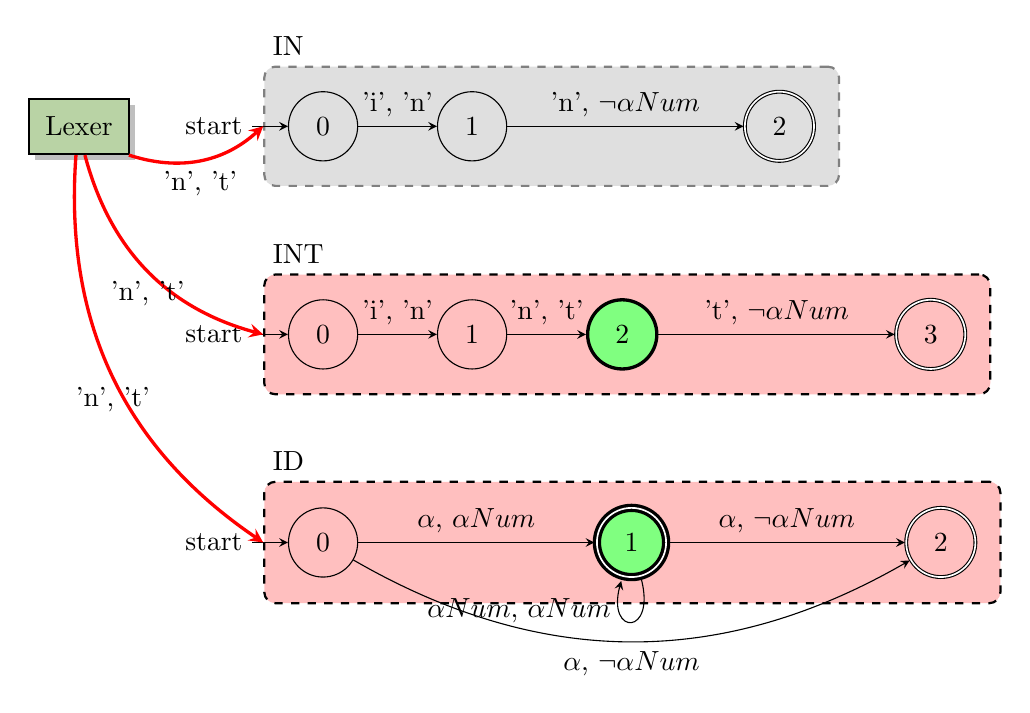
\begin{tikzpicture}[auto,
    ->,
    >=stealth,
    ,
    dead/.style={%
      rectangle, rounded corners=1.5mm, draw=gray, thick, fill=gray!25, drop shadow,align=center,
      text ragged, minimum height=2em, minimum width=2em, inner sep=6pt, outer sep=3pt
    },
    fun/.style = {%
      dashed, draw=black, thick, fill=red!25, rounded corners, rectangle, inner sep=.3cm
    },
    deadfun/.style = {%
      dashed, draw=gray, thick, fill=gray!25, rounded corners, rectangle, inner sep=.3cm
    }
  ]

    \node[bb] (lexer)                           {Lexer};
% IN  
    \node[initial, state]   (10) [right = of lexer, xshift=1cm]          {$0$};
    \node[state]            (11) [right = of 10]             {$1$};
    \node[state, accepting] (12) [right = of 11, xshift=2cm] {$2$};
    
    \path (10) edge node {'i', 'n'} (11)
          (11) edge node {'n', $\neg\alpha Num$} (12)
    ;

% INT
    \node[initial, state]   (20) [below = of 10, yshift = -0.75cm] {$0$};
    \node[state]            (21) [right = of 20] {$1$};
    \node[state, very thick, fill=green!50]            (22) [right = of 21] {$2$};
    \node[state, accepting] (23) [right = of 22, xshift=2cm] {$3$};
    
    \path (20) edge node {'i', 'n'} (21)
          (21) edge node {'n', 't'} (22)
          (22) edge node {'t', $\neg\alpha Num$} (23)
    ;
    
%ID
    \node[initial, state]   (30) [below = of 20, yshift = -0.75cm] {$0$};
    \node[state, accepting, very thick, fill=green!50]            (31) [right = of 30, xshift=2cm] {$1$};
    \node[state, accepting]            (32) [right = of 31, xshift=2cm] {$2$};
    
    \path (30) edge node {$\alpha$, $\alpha Num$} (31)
              (31) edge[loop below] node[near end, left] {$\alpha Num$, $\alpha Num$} (31)
              (31) edge node[above] {$\alpha$, $\neg\alpha Num$} (32)
          (30) edge[bend right] node[below] {$\alpha$, $\neg\alpha Num$} (32)
    ;
    
    \begin{pgfonlayer}{background}
      \node[deadfun] (in)[fit = (10) (11) (12)] {};
      \node[fun] (int)[fit = (20) (21) (22) (23)] {};
      \node[fun] (id)[fit = (30) (31) (32)] {};
      \node[above right] at (in.north west){IN};
      \node[above right] at (int.north west){INT};
      \node[above right] at (id.north west){ID};

    \end{pgfonlayer}
    
	\draw[->, very thick, red, bend right] (lexer) to node[below, black]{'n', 't'} (in.west);
	\draw[->, very thick, red, bend right] (lexer) to node[below, black]{'n', 't'} (int.west);
	\draw[->, very thick, red, bend right] (lexer) to node[below, black]{'n', 't'} (id.west);
	    
  \end{tikzpicture}
}

\end{center}

\end{frame}
% frame end %%%%%%%%%%%%%%%%%%%%%%%%

% frame begin %%%%%%%%%%%%%%%%%%%%%%%%
\begin{frame}{Implementation of Lexical Analysis}
{Manual Implementation of Lexical Analysers -- Example}
\begin{center}
\begin{tabular}{|c|c|c|c|c|c|c|c|}
\hline
i & n & \cellcolor{red!75}t & \cellcolor{red!25}e & g & r & a & l \\
\hline
\end{tabular}
\end{center}

\begin{center}
\resizebox{0.7\textwidth}{!}{%
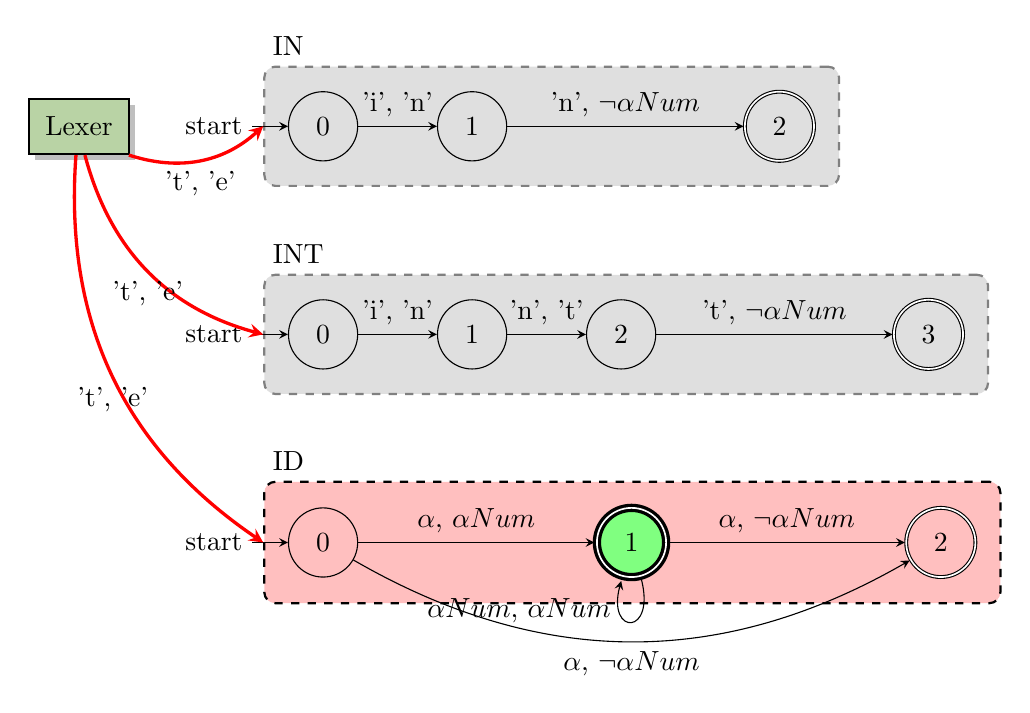
\begin{tikzpicture}[auto,
    ->,
    >=stealth,
    ,
    dead/.style={%
      rectangle, rounded corners=1.5mm, draw=gray, thick, fill=gray!25, drop shadow,align=center,
      text ragged, minimum height=2em, minimum width=2em, inner sep=6pt, outer sep=3pt
    },
    fun/.style = {%
      dashed, draw=black, thick, fill=red!25, rounded corners, rectangle, inner sep=.3cm
    },
    deadfun/.style = {%
      dashed, draw=gray, thick, fill=gray!25, rounded corners, rectangle, inner sep=.3cm
    }
  ]

    \node[bb] (lexer)                           {Lexer};
% IN  
    \node[initial, state]   (10) [right = of lexer, xshift=1cm]          {$0$};
    \node[state]            (11) [right = of 10]             {$1$};
    \node[state, accepting] (12) [right = of 11, xshift=2cm] {$2$};
    
    \path (10) edge node {'i', 'n'} (11)
          (11) edge node {'n', $\neg\alpha Num$} (12)
    ;

% INT
    \node[initial, state]   (20) [below = of 10, yshift = -0.75cm] {$0$};
    \node[state]            (21) [right = of 20] {$1$};
    \node[state]            (22) [right = of 21] {$2$};
    \node[state, accepting] (23) [right = of 22, xshift=2cm] {$3$};
    
    \path (20) edge node {'i', 'n'} (21)
          (21) edge node {'n', 't'} (22)
          (22) edge node {'t', $\neg\alpha Num$} (23)
    ;
    
%ID
    \node[initial, state]   (30) [below = of 20, yshift = -0.75cm] {$0$};
    \node[state, accepting, very thick, fill=green!50]            (31) [right = of 30, xshift=2cm] {$1$};
    \node[state, accepting]            (32) [right = of 31, xshift=2cm] {$2$};
    
    \path (30) edge node {$\alpha$, $\alpha Num$} (31)
          (31) edge[loop below] node[near end, left] {$\alpha Num$, $\alpha Num$} (31)
          (31) edge node[above] {$\alpha$, $\neg\alpha Num$} (32)
          (30) edge[bend right] node[below] {$\alpha$, $\neg\alpha Num$} (32)
    ;
    
    \begin{pgfonlayer}{background}
      \node[deadfun] (in)[fit = (10) (11) (12)] {};
      \node[deadfun] (int)[fit = (20) (21) (22) (23)] {};
      \node[fun] (id)[fit = (30) (31) (32)] {};
      \node[above right] at (in.north west){IN};
      \node[above right] at (int.north west){INT};
      \node[above right] at (id.north west){ID};

    \end{pgfonlayer}
    
	\draw[->, very thick, red, bend right] (lexer) to node[below, black]{'t', 'e'} (in.west);
	\draw[->, very thick, red, bend right] (lexer) to node[below, black]{'t', 'e'} (int.west);
	\draw[->, very thick, red, bend right] (lexer) to node[below, black]{'t', 'e'} (id.west);
	    
  \end{tikzpicture}
}

\end{center}

\end{frame}
% frame end %%%%%%%%%%%%%%%%%%%%%%%%

% frame begin %%%%%%%%%%%%%%%%%%%%%%%%
\begin{frame}{Implementation of Lexical Analysis}
{Manual Implementation of Lexical Analysers -- Example}
\begin{center}
\begin{tabular}{|c|c|c|c|c|c|c|c|}
\hline
i & n & t & e & g & r & a & \cellcolor{red!75}l \\
\hline
\end{tabular}
\end{center}

\begin{center}
\resizebox{0.7\textwidth}{!}{%
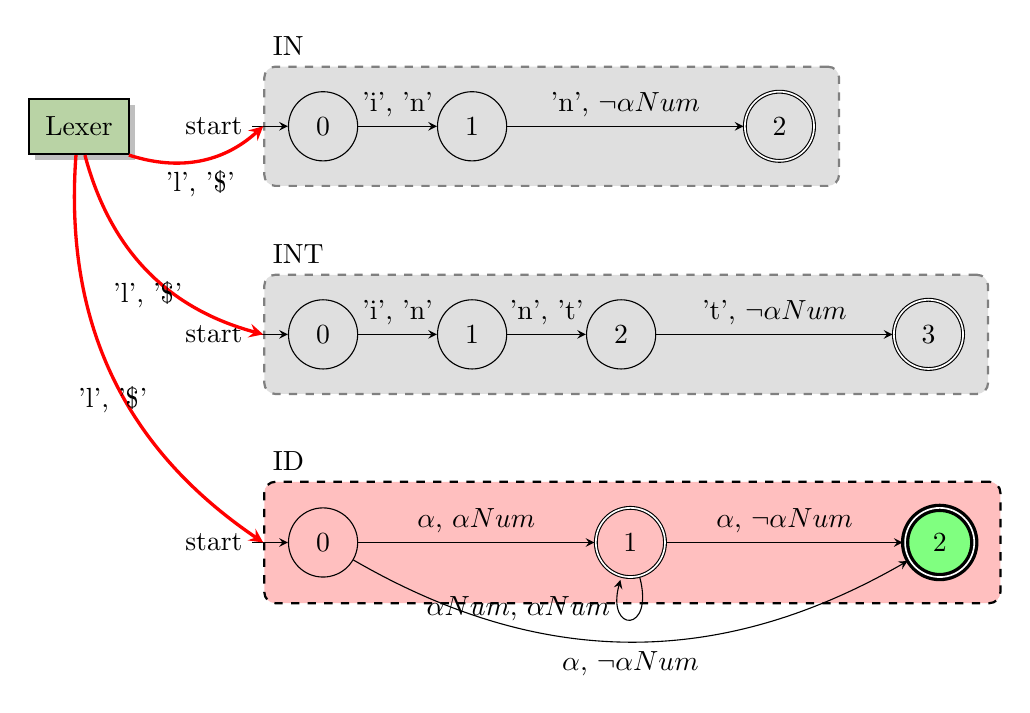
\begin{tikzpicture}[auto,
    ->,
    >=stealth,
    ,
    dead/.style={%
      rectangle, rounded corners=1.5mm, draw=gray, thick, fill=gray!25, drop shadow,align=center,
      text ragged, minimum height=2em, minimum width=2em, inner sep=6pt, outer sep=3pt
    },
    fun/.style = {%
      dashed, draw=black, thick, fill=red!25, rounded corners, rectangle, inner sep=.3cm
    },
    deadfun/.style = {%
      dashed, draw=gray, thick, fill=gray!25, rounded corners, rectangle, inner sep=.3cm
    }
  ]

    \node[bb] (lexer)                           {Lexer};
% IN  
    \node[initial, state]   (10) [right = of lexer, xshift=1cm]          {$0$};
    \node[state]            (11) [right = of 10]             {$1$};
    \node[state, accepting] (12) [right = of 11, xshift=2cm] {$2$};
    
    \path (10) edge node {'i', 'n'} (11)
          (11) edge node {'n', $\neg\alpha Num$} (12)
    ;

% INT
    \node[initial, state]   (20) [below = of 10, yshift = -0.75cm] {$0$};
    \node[state]            (21) [right = of 20] {$1$};
    \node[state]            (22) [right = of 21] {$2$};
    \node[state, accepting] (23) [right = of 22, xshift=2cm] {$3$};
    
    \path (20) edge node {'i', 'n'} (21)
          (21) edge node {'n', 't'} (22)
          (22) edge node {'t', $\neg\alpha Num$} (23)
    ;
    
%ID
    \node[initial, state]   (30) [below = of 20, yshift = -0.75cm] {$0$};
    \node[state, accepting]            (31) [right = of 30, xshift=2cm] {$1$};
    \node[state, accepting, very thick, fill=green!50]            (32) [right = of 31, xshift=2cm] {$2$};
    
    \path (30) edge node {$\alpha$, $\alpha Num$} (31)
          (31) edge[loop below] node[near end, left] {$\alpha Num$, $\alpha Num$} (31)
          (31) edge node[above] {$\alpha$, $\neg\alpha Num$} (32)
          (30) edge[bend right] node[below] {$\alpha$, $\neg\alpha Num$} (32)
	;
	    
    \begin{pgfonlayer}{background}
      \node[deadfun] (in)[fit = (10) (11) (12)] {};
      \node[deadfun] (int)[fit = (20) (21) (22) (23)] {};
      \node[fun] (id)[fit = (30) (31) (32)] {};
      \node[above right] at (in.north west){IN};
      \node[above right] at (int.north west){INT};
      \node[above right] at (id.north west){ID};

    \end{pgfonlayer}
    
	\draw[->, very thick, red, bend right] (lexer) to node[below, black]{'l', '\$'} (in.west);
	\draw[->, very thick, red, bend right] (lexer) to node[below, black]{'l', '\$'} (int.west);
	\draw[->, very thick, red, bend right] (lexer) to node[below, black]{'l', '\$'} (id.west);
	    
  \end{tikzpicture}
}

\end{center}

\end{frame}
% frame end %%%%%%%%%%%%%%%%%%%%%%%%

% frame begin %%%%%%%%%%%%%%%%%%%%%%%%
\begin{frame}{Implementation of Lexical Analysis}
{Manual Implementation of Lexical Analysers -- Example}
\begin{center}
\resizebox{!}{0.7\textheight}{%
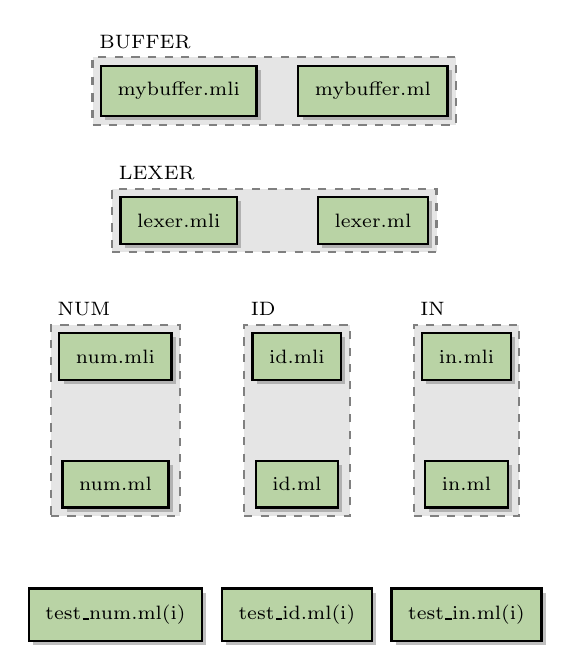
\begin{tikzpicture}[auto,
    ->,
    >=stealth,
    ]
\begin{scriptsize}

    \node[bb] (num_mli)   {num.mli};
    \node[bb, below=of num_mli]   (num_ml)    {num.ml};

    \node[bb, right=of num_mli]   (id_mli)    {id.mli};
    \node[bb, below=of id_mli]    (id_ml)     {id.ml};
	    
    \node[bb, right=of id_mli]    (in_mli)    {in.mli};
    \node[bb, below=of in_mli]    (in_ml)     {in.ml};

    \node[bb, below=of num_ml]   (tnum_ml)    {test\_num.ml(i)};

    \node[bb, below=of id_ml]    (tid_ml)     {test\_id.ml(i)};
	    
    \node[bb, below=of in_ml]    (tin_ml)     {test\_in.ml(i)};

    \begin{pgfonlayer}{background}
      \node[draw=Gray, dashed, thick, fill=Gray!20] (num)[fit = (num_mli) (num_ml)] {};
      \node[above right] (lnum) at (num.north west){NUM};

      \node[draw=Gray, dashed, thick, fill=Gray!20] (id)[fit = (id_mli) (id_ml)] {};
      \node[above right] (lid) at (id.north west){ID};

      \node[draw=Gray, dashed, thick, fill=Gray!20] (in)[fit = (in_mli) (in_ml)] {};
      \node[above right] (lin) at (in.north west){IN};

	\end{pgfonlayer}    

    \node[bb, above= of id, xshift=-1.5cm]                     (lexer_mli) {lexer.mli};
    \node[bb, right=of lexer_mli] (lexer_ml)  {lexer.ml};

    \begin{pgfonlayer}{background}
      \node[draw=Gray, dashed, thick, fill=Gray!20] (lexer)[fit = (lexer_mli) (lexer_ml)] {};
      \node[above right] (llexer) at (lexer.north west){LEXER};
	\end{pgfonlayer}    


    \node[bb, above= of lexer_mli]                     (mybuffer_mli) {mybuffer.mli};
    \node[bb, above=of lexer_ml] (mybuffer_ml)  {mybuffer.ml};

    \begin{pgfonlayer}{background}
      \node[draw=Gray, dashed, thick, fill=Gray!20] (mybuffer)[fit = (mybuffer_mli) (mybuffer_ml)] {};
      \node[above right] (lmybuffer) at (mybuffer.north west){BUFFER};
	\end{pgfonlayer}    

\end{scriptsize}
  \end{tikzpicture}
}

\end{center}

\end{frame}
% frame end %%%%%%%%%%%%%%%%%%%%%%%%


% frame begin %%%%%%%%%%%%%%%%%%%%%%%%
\begin{frame}[fragile]{Manual Implementation of Lexical Analysis}
{Lazy implementation}
\begin{enumerate}
	\item FSA: Pair of \emph{current state} and \emph{list of accepting states}
\begin{lstlisting}[style=camlcode]
let id () : State.state * 
  ((char -> char option -> State.state) list) =
\end{lstlisting}

	\item State $\mapsto$ Mutually recursive higher order function
\begin{lstlisting}[style=camlcode]
let rec one (c : char) (lookahead : char option) 
  : State.state =
  ...
  ...
and two  (c : char) (lookahead : char option)
  : State.state =
\end{lstlisting}
	\item Takes two characters as input: \emph{current character} and \emph{lookahead} ($\Sigma' = \Sigma \times \Sigma$)
\end{enumerate}
\end{frame}
% frame end %%%%%%%%%%%%%%%%%%%%%%%%

% frame begin %%%%%%%%%%%%%%%%%%%%%%%%
\begin{frame}[fragile]{Manual Implementation of Lexical Analysis}
{State}
\texttt{\color{Brown}state.mli}
\begin{lstlisting}[style=camlcode]
type state =
    Terminate of bool
  | State of (char -> char option -> state)
\end{lstlisting}

\begin{enumerate}
	\item Models the return type of a state function
	\item \hspace{1cm}
	
	\begin{quotation}
	Terminate in failure (\lstinline[style=camlcode]|false|) or success (\lstinline[style=camlcode]|true|)
	
	OR
	
	Next state
	\end{quotation}
	\item Caller can decide if/when/how to explore the next state
\end{enumerate}
\end{frame}
% frame end %%%%%%%%%%%%%%%%%%%%%%%%

% frame begin %%%%%%%%%%%%%%%%%%%%%%%%
\begin{frame}[fragile]{Manual Implementation of Lexical Analysis}
{Buffer}
\texttt{\color{Brown}mybuffer.mli}
\begin{lstlisting}[style=camlcode]
exception End_of_buffer
val from_string : bytes -> (unit -> (char * char option))
val from_file : bytes -> (unit -> char -> char option)
\end{lstlisting}

\texttt{\color{Brown}mybuffer.ml}
\begin{lstlisting}[style=camlcode]
let from_file fname =
  ...
  let buffer () : (char * char option) =
    ...
    
  in
  buffer
\end{lstlisting}

\begin{enumerate}
	\item Represents the input source
	
	\item Stateful
	\item Caller can decide if/when/how to explore the next state
\end{enumerate}
\end{frame}
% frame end %%%%%%%%%%%%%%%%%%%%%%%%


% frame begin %%%%%%%%%%%%%%%%%%%%%%%%
\begin{frame}[fragile]{Manual Implementation of Lexical Analysis}
{Source code}

\begin{scriptsize}

\begin{enumerate}
\item Buffer
\item FSAs (NUM, ID, IN)
\item Lexer
\item Makefile
\end{enumerate}
\end{scriptsize}
\end{frame}
% frame end %%%%%%%%%%%%%%%%%%%%%%%%

\end{document}
